\chapter{The Functional Therapeutic Chemical Classification System (Implementation)}

\textbf{Key points}
\begin{itemize}
  \item New mode and mechanism of action (MoA) concepts can be formally created using description logics and following the principles introduced in Chapter 2.
  \item 20,000 new MoA concepts are created and present in a novel resource called the Functional Therapeutic Chemical Classification System (FTC). The resource has a taxonomic structure and describes the biological roles of drugs (e.g. anti-blood coagulation agent).
  \item Over a thousand of approved drugs are classified inside the FTC categories by integrating the content of DrugBank, UniProt and Gene Ontology Annotations (GOA) and with the help of an OWL reasoner. The classification process is fast and complete, as the axioms present in the FTC follow the EL++ profile.
  \item The biomedical information present in the FTC is evaluated against the content of the Anatomical Therapeutic Chemical Classification System (ATC), manually curated resource describing the indication, function and therapeutic areas of approved drugs. Briefly, the drugs classified in the FTC are covering 89\% of the content of the ATC (recall). Given a therapeutic category, the FTC contains more drugs than the ATC, reflecting the drug’s polypharmacology (precision of 50\%).
  \item The content of the FTC will be used to derive systematic drug repositioning hypotheses as presented in Chapter 4.
\end{itemize}

\textbf{Author's comment}

The content and structure of this chapter were directly extracted from the published article \citep{croset2013functional} describing the FTC and some of the analyses performed over it. I have edited the text in order to provide more details when needed and relevant, and to hopefully keep the coherence with the rest of the document. The argumentation has a classical structure: The methodology behind the creation of the resource is first presented, followed by an evaluation section. The results obtained are finally contrasted and discussed.

\hrulefill

\section{Introduction}
Chapter 1 introduced my thesis, namely formally representing drug’s mechanisms and modes of action in order to discover new indications. In Chapter 2 was presented a theoretical perspective on description logics (DLs) and their relation to the study of life. This chapter implements the theory and describes the generation and evaluation of mode of action categories.

As stated in Chapter 1, drug repurposing is the use of known active compounds for new therapeutic indications \citep{sanseau2011editorial}. When administered in a living organism, a compound can indeed play various roles and affect different biological processes; accurately identifying these different functions helps to predict the potential side-effects a drug can have and can also lead to interesting repositioning opportunities \citep{medina2013shifting}. For instance, \emph{sildenafil} was initially developed to relieve angina pectoris symptoms and has been repurposed towards erectile dysfunction during the clinical trials \citep{ashburn2004drug} when a new function of the target enzyme was discovered (see Chapter 1). 

Approved compounds are attractive because they have been extensively studied and have by definition already successfully passed clinical trials, where most drugs fail because of safety or efficacy issues. There is an increasing number of approaches to predict repurposing opportunities using computational methods (see Chapter 1). Most methods operate on the profiles of physicochemical descriptors derived from molecular structures \citep{haupt2011old}. Other methods characterise the drugs on more abstract levels, such as the gene expression signature \citep{iorio2010discovery} or via the reported side-effects \citep{campillos2008drug}. These approaches have in common to look for similarities within existing drugs and forward similar compounds as repurposing hypotheses.

A feature of particular interest to describe drugs is the MoA. According to Wikipedia, the MoA describes \emph{a functional or anatomical change, at the cellular level, resulting from the exposure of a living organism to a substance}. For instance terms such as \emph{transcriptional regulation agent} or \emph{anticoagulant} define MoAs and characterise the roles of a certain type of drug. The MoA abstracts over the relations between molecular functions, protein targets and drug activities; it is the central concept linking a chemical structure to a set of biological activities (see Chapter 1). Intuitively, the indication of a drug logically depends on its MoA (see Figure \ref{fig3-1}).

\begin{figure}[ht]
    \centering
    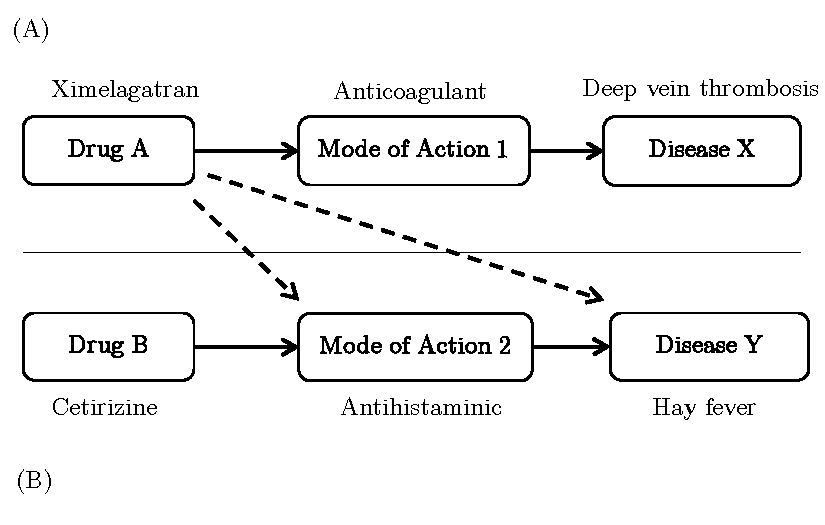
\includegraphics{fig3-1}
    \caption{Conceptual relationship between a drug, its mode of action (MoA) and disease indication. Because a drug exhibits a certain MoA it is therefore indicated for a diseases, as showed by examples (A) and (B). If a new MoA was discovered for a drug (e.g. ximelagatran with antihistaminic MoA), the compound could be re-indicated accordingly (in this case for hay fever – illustrated by the dashed arrows). In order for such a deduction to be made, MoA categories first have to be represented, and secondly drugs have to be assigned to these categories.}
    \label{fig3-1}
\end{figure}

Despite its widespread use in drug discovery, the MoA has not been used yet as a descriptor for repositioning analyses. One reason for this might be the challenge of formally defining the concept. Indeed, MoAs are terms or categories, it is not possible to represent them straightforwardly with values and numbers like one can do for a 3D molecular structure or for a gene expression profile. Nonetheless, the meaning of a concept can be formalised with controlled vocabularies and ontologies \citep{gruber2009encyclopedia}; such frameworks help to formalise the semantics of symbols and strings of characters with explicit axioms (see Chapter 2). 

In an ontology or knowledge base, concepts (interchangeable with \emph{category}, \emph{term} and \emph{class} in this document) are organised and linked following the logical type of relation they have among them. In the Gene Ontology (GO) for example \citep{ashburner2000gene}, biological processes and molecular functions terms are manually curated  and their meaning specified by the relation types linking two GO terms. MoA definitions are present in other classifications such as the Medical Subject Headings \citep{nelson2004mesh} or the Chemical Entities of Biological Interest \citep{hastings2013chebi}. The Anatomical Therapeutic Chemical Classification System (ATC) \citep{world2006anatomical} also describes to some extent the action of drugs at the anatomical level. All these resources are valuable for the community as a source of carefully manually curated information. Moreover, the categories described in these classification systems are sometimes used to annotate drugs: For instance the compound \emph{sildenafil} has been manually annotated as \emph{vasodilator agent} (CHEBI:35620 or MeSH:D27.505.954.411.918).

The classifications mentioned previously are not specially designed for drug repositioning; they purposefully report only the well-known and major MoAs of chemical compounds. The pharmacological spectrum of each drug is not necessarily well covered, yet it would be the best way to predict new indications. In my context, an ideal knowledge base would feature the known MoAs of a drug as well as some predicted ones to be tested in experiments. The MoA categories should derive and scale over primary molecular evidence exposed in biomedical databases, in an automated way as motivated in Chapter 2.

To address the lack of systematic MoA annotations, I have implemented the Functional Therapeutic Chemical Classification System (FTC), presented here in this chapter. The FTC is automatically built by leveraging the content of various biomedical databases using description logics and automated reasoning. Over 20,000 new MoA categories are defined in the resource and further populated with approved drugs using the Web Ontology Language (OWL) in combination with a reasoner. The population step takes in account the type of pharmacological action, the molecular targets of the drugs and their involvement into multiple biological processes.

Drugs can exhibit several MoAs, and the same MoA can be reached through different mechanisms. Most of the drugs are present in multiple FTC categories, reflecting the various roles a compound can play inside a biological system which can serve as starting point for drug repositioning. The resource was evaluated against the ATC, traditional classification scheme introduced before. I present as well some preliminary analyses over the data, by looking at the relation between the MoA and the indication of a compound using semantic similarity. Finer analyses and repositioning use-cases such as Alzheimer’s disease and hypertension will be investigated in Chapter 4.

\section{Method and definitions}
This section describes the building mechanism behind the FTC. The full list of axioms composing the knowledge base are listed at the end of this section (//ref section specification). The FTC is one possible implementation of the theory described in Chapter 2, dedicated to handle MoAs.

Summarised, the creation of the FTC follows these steps: First, a list of categories describing the mode and mechanism of action of drugs is defined. Then in a second step the newly created categories are automatically populated with approved compounds. Finally, the FTC is evaluated and repositioning hypotheses can be generated (presented in Chapter 4).

\subsection{Source code}
The code behind the creation of the resource is entirely open and available at {{https://github.com/loopasam/ftc}}. The web application built on the top of the FTC can be found at {{https://www.ebi.ac.uk/chembl/ftc}} and the documentation can be accessed at {{https://github.com/loopasam/ftc/wiki}}. The reader should be familiar with DLs and the Web Ontology Language (OWL) to fully understand the construction of the knowledge base. An introduction to description logics from the perspective of the biomedical scientist is available on the wiki at {{https://github.com/loopasam/ftc/wiki/Description-Logics}} and in Chapter 2 section. The FTC implementation relies mostly on Brain \citep{croset2013brain} and the web application builds on the top of the Play! framework ({{http://www.playframework.com/}}). Classification tasks use the ELK reasoner \citep{kazakov2013incredible}. The computer hosting the web application has 8 Gb of memory with 4 processors, this architecture allows fast parallel reasoning, thanks to ELK's design. More functionalities will be added to the web application following user requirements (\emph{lean implementation}).

\subsection{Categories creation}
\label{catfunc}

The mode of action categories present in the FTC are defined based on the terms coming from the Gene Ontology (GO). Both the molecular function and biological process branches are used for this purpose, yet handled slightly differently as described below.

\subsubsection{Mode of Action categories}
All the biological processes featured in the GO are looked-up one by one. All the time a process is linked to another process (\emph{X}) via a \emph{positive} or \emph{negative regulation} link, two FTC classes are created: \emph{Anti-X agent} and \emph{Pro-X agent}. For instance the GO term \emph{positive regulation of blood coagulation} is linked to the term \emph{blood coagulation} via a \emph{positively regulates} relation, therefore two FTC categories \emph{Anti-blood coagulation agent} and \emph{Pro-blood coagulation agent} are created. The identifiers of the new FTC classes are also derived from the GO term used to create the class pattern. The GO numeric identifier is re-used and the letter \emph{A} or \emph{P} is appended before to emphasize the \emph{anti} or \emph{pro} pattern. From the example presented previously, the FTC class \emph{Anti-blood coagulation} has FTC\_A0007596 as identifier, because the GO term \emph{blood coagulation} is referenced as GO:0007596. Following the same logic, FTC\_P0007596 is the identifier of the class \emph{Pro-blood coagulation agent}. The design choice for identifiers and labels allows the FTC to fully rely on the high quality work provided by the GO curation team and scale over it.

\subsubsection{Mechanism of Action categories}
The mechanism of actions related to molecular functions are created in the following manner: All the time a molecular function (\emph{Y}) is encountered then two FTC categories are created, as for the processes: \emph{Anti-Y agent} and \emph{Pro-Y agent}. The identifiers are assigned the same way as described before. For instance, out of the GO term \emph{androgen receptor activity} (GO:0004882) two FTC classes are derived: \emph{Pro-androgen receptor activity agent} (FTC\_P0004882) and \emph{Anti-androgen receptor activity agent} (FTC\_A0004882).

\subsection{Equivalent definitions}
FTC classes are generated as presented in the previous section. Up to this point, these categories are only tokens with a human readable label as well as an identifier. The next step is going to assign equivalent definitions to each FTC class. An OWL reasoner can understand such definitions and will automatically classify the knowledge base accordingly, following standard description logics reasoning services (see Chapter 2 section).
Drugs will then be assigned to FTC categories and the taxonomic structure arises after this reasoning step. Equivalent definitions are written as OWL class expressions using the entities of the knowledge base (summarised at {{https://github.com/loopasam/ftc/wiki/Knowledge-Base}} and in section \ref{specs}). There are two types of equivalences: The first one captures perturbation of regulatory biological processes (so called \emph{regulatory patterns}) and the second one handles the perturbed functions (\emph{functional patterns}).

\subsubsection{Regulatory pattern}
Some of the FTC categories are created from the biological processes present in the GO (cf section \ref{catprocess}); these categories have two arbitrary equivalent definitions, representing the two possible ways a compound might impact the biological process. Anti-biological process agent FTC categories contain the drugs that negatively perturb a target involved in the positive regulation of the biological process. The \emph{anti} categories also feature the compounds that positively perturb a negative regulator of the same process. The \emph{pro} categories are equivalent to the opposite pattern. Figure \ref{fig3-2} and \ref{fig3-3} illustrates the equivalent definitions for the FTC classes \emph{Anti-blood coagulation agent} and \emph{Anti-blood coagulation agent}.

\begin{figure}[ht]
    \centering
    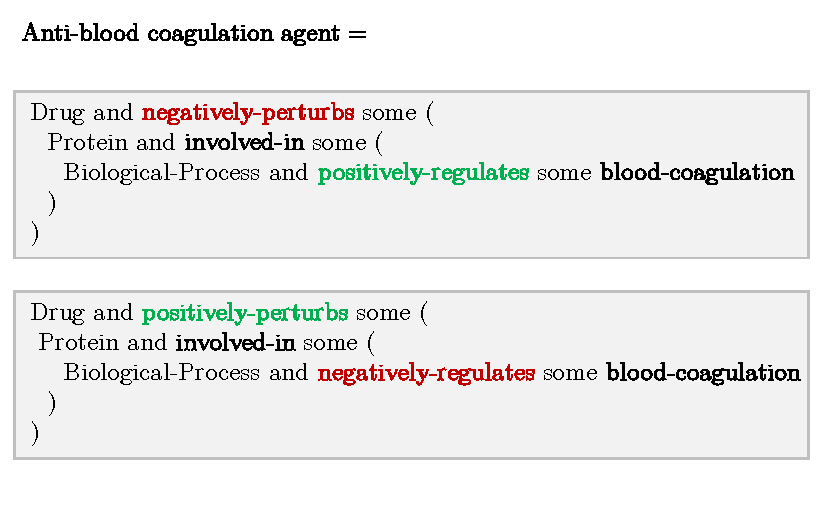
\includegraphics{fig3-2}
    \caption{Regulatory pattern. Equivalent definitions for the concept “Anti-blood coagulation agent”. The concept is asserted as equivalent to either of the boxed expressions. A reasoner can understand such definition and classify drugs accordingly.}
    \label{fig3-2}
\end{figure}

\begin{figure}[ht]
    \centering
    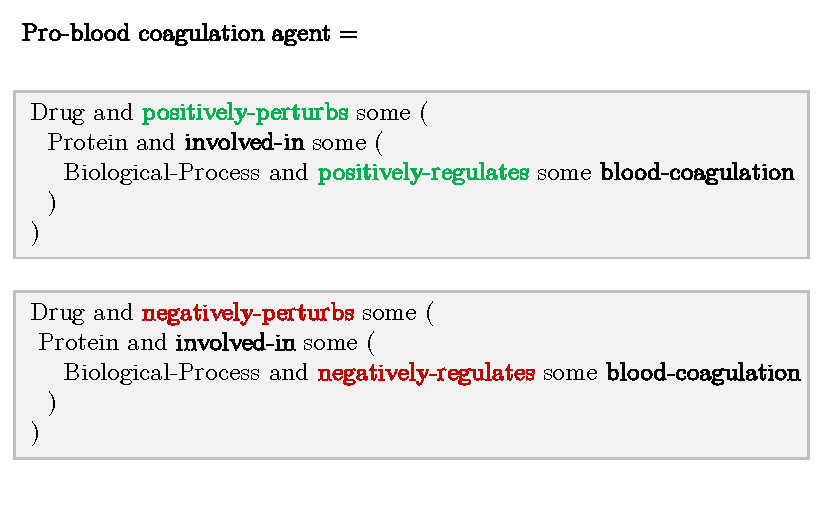
\includegraphics{fig3-3}
    \caption{Example of regulatory pattern. Equivalent definitions for the concept “Pro-blood coagulation agent”. The concept is asserted as equivalent to either of the boxed expressions. A reasoner can understand such definition and classify drugs accordingly.}
    \label{fig3-3}
\end{figure}

Figures \ref{fig3-4} and \ref{fig3-5} present the biological motivation behind the regulatory patterns: it should be easier to adjust the dosage for the compounds classified as such.

\begin{figure}[ht]
    \centering
    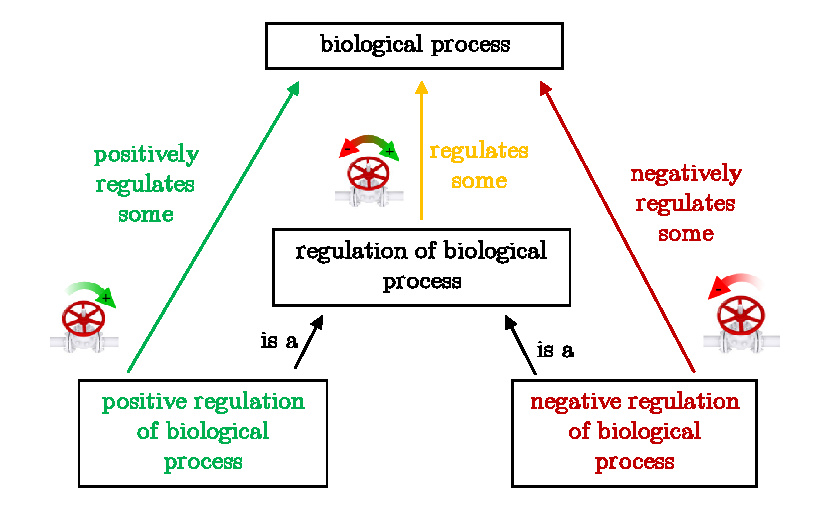
\includegraphics{fig3-4}
    \caption{Biological processes of therapeutic interest are perturbed via regulators of the given process; this strategy allows to modulate and tune the effect, rather than blocking it totally. A regulatory process can be seen as a valve controlling the amplitude or frequency of another process, as defined in the Gene Ontology. This characteristic is of interest for drug discovery, it means that the strength of the pharmacological effect is more likely adaptable with the dosage and drug’s concentration.}
    \label{fig3-4}
\end{figure}

\begin{figure}[ht]
    \centering
    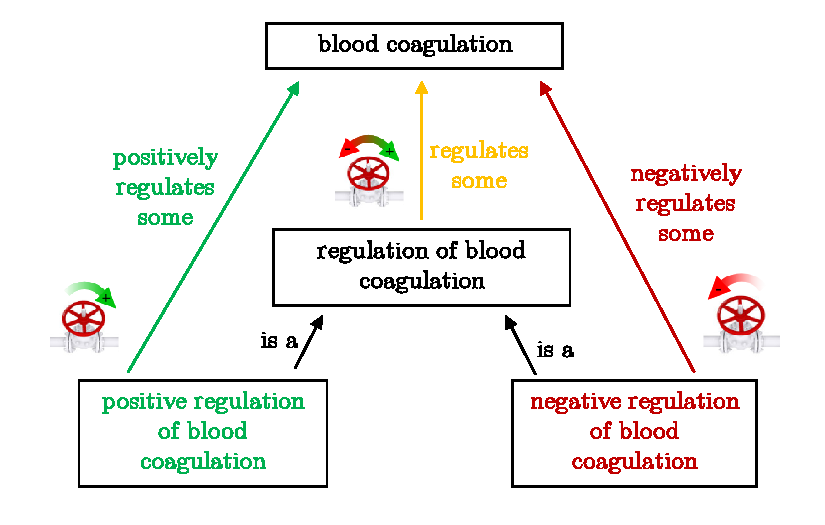
\includegraphics{fig3-5}
    \caption{Example of regulation of the blood coagulation process, as defined in the Gene Ontology. Perturbing the coagulation via a regulator allows to more finely control the therapeutic outcome. See Figure \ref{fig3-4} for theoretical illustration.}
    \label{fig3-5}
\end{figure}

\subsubsection{Functional pattern}
The FTC categories generated from the GO molecular functions (cf section \ref{catfunc}) are also equivalent to a logical definition. \emph{Anti} FTC categories dealing with molecular activities are asserted as equals to the drugs that negatively perturb the function. \emph{Pro} categories are equivalent to the drugs that positively perturb the function of interest. A summary of the functional pattern definitions is available on the online wiki at {{https://github.com/loopasam/ftc/wiki/Mode-of-Action}} and on Figure \ref{fig3-6}.

\begin{figure}[ht]
    \centering
    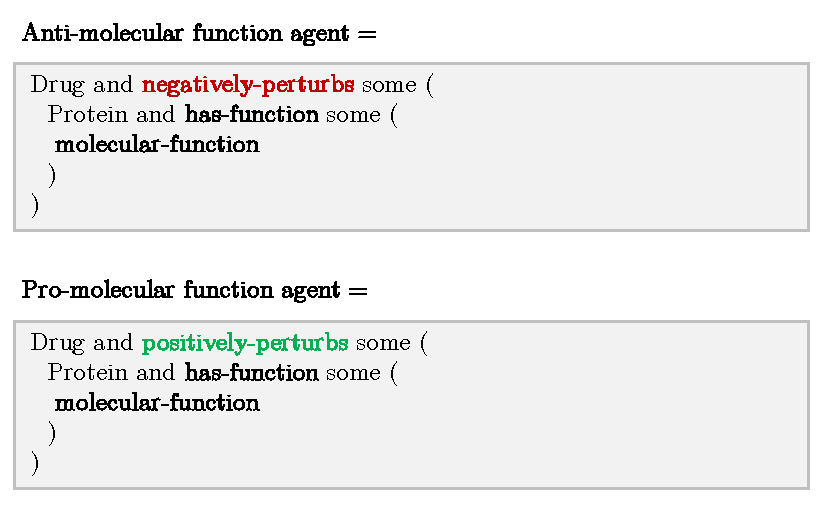
\includegraphics{fig3-6}
    \caption{Example of functional patterns; equivalent definitions for the concepts “pro and anti-molecular function agent”. These concepts is asserted as equivalent to either of the boxed expressions. A reasoner can understand such definition and classify drugs accordingly.}
    \label{fig3-6}
\end{figure}
s
